\begin{figure*}
 \centering
 \begin{minipage}[t]{0.43\linewidth}
 \centering
 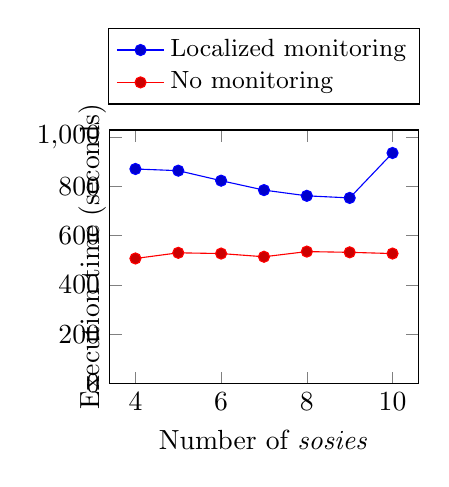
\begin{tikzpicture}
  \begin{axis}[
  	ylabel={Execution time (seconds)},
  	y label style={at={(0.02, 0.5)}},
  	legend style={at={(0.5,1.1)},
  	 	 	anchor=south,legend columns=1, font=\small},
  	ymin=0,
  	every axis legend/.append style={nodes={right}},
  	xlabel={Number of \textit{sosies}},width = 5.5cm,
  	height = 4.8cm]
 
  \addplot+[mark=*] coordinates
  	{(4, 870.375) (5, 863.5) (6, 822.875) (7, 784.625) (8, 761.375) (9, 752.875) (10, 935.3)};

\addplot+[mark=*] coordinates
  	{(4, 507) (5, 530) (6, 527) (7, 514) (8, 535) (9, 532) (10, 527)};
  	
  	\legend{Localized monitoring, No monitoring}
  	
  \end{axis}
  \end{tikzpicture}
  \caption{Time to obtain the reply to all requests.\label{fig:execution-time-web-app}}
  \end{minipage}
  \hspace{0.1\linewidth}
 \begin{minipage}[t]{0.43\linewidth}
 \centering
 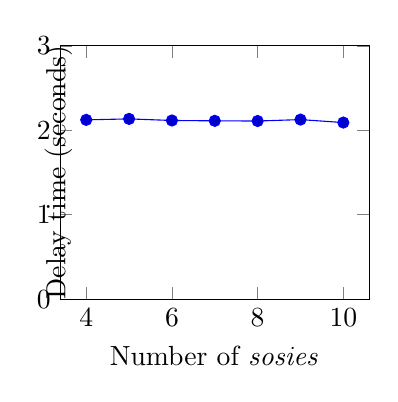
\begin{tikzpicture}
 \begin{axis}[
 	ylabel={Delay time (seconds)},
 	y label style={at={(0.07, 0.5)}}, 	
 	ymin=0,ymax=3,
 	xlabel={Number of \textit{sosies}},width = 5.5cm,
 	height = 4.8cm]

 \addplot+[mark=*] coordinates
 	{(4,2.1235) (5, 2.1348) (6,2.11605) (7,2.1119) (8, 2.1097) (9, 2.12654) (10, 2.09139)};
 	
 \end{axis}
 \end{tikzpicture}
 \caption{Average delay time to detect a faulty \textit{sosie}.\label{fig:delay-time-web-app}}
\end{minipage}

\hspace{1cm}
\end{figure*}
